%%
% BIThesis Undergraduate Thesis Template (English) — Compile with XeLaTeX
% Chapter 2: System Architecture
%%

\chapter{System Architecture}

This chapter presents the complete system architecture for the SDN global control plane. It details the microservice layout, the asynchronous decoupling strategy, and the specific data workflows that enable the dynamic bandwidth marketplace. By moving away from monolithic controller designs, this architecture ensures high availability and scalability, though it introduces significant distributed tracking challenges that necessitate a custom observability framework.

\section{Architectural Overview}

The complete architecture of the SDN global control plane is illustrated in Figure~\ref{fig:full_architecture}. The system is organized into three primary microservices: customer request handling (API Gateway), resource allocation (Auction Runner), and measurement aggregation (Telemetry Processor). 

As shown in the figure, these services do not communicate directly via synchronous remote procedure calls (RPCs). Instead, they interact through a state-separated architecture utilizing a shared consensus store (Atomix) and an asynchronous message broker (Apache Kafka).

\begin{figure}[H]
  \centering
  
\includegraphics[width=0.95\textwidth]{images/full-fyp-architecture.pdf}
  \caption{System architecture of the observable SDN global control plane, illustrating the separation of state and asynchronous event routing.}
  \label{fig:full_architecture}
\end{figure}

Customer bids flow into the API Gateway and are written directly to Atomix, ensuring immediate consistency across replicas. At scheduled intervals, the Auction Runner pulls these bids, computes allocations, and pushes results to Kafka. Finally, the simulated data-plane agents consume these allocations while simultaneously publishing flow statistics back to Kafka, which the Telemetry Processor ingests.

\section{Asynchronous Decoupling via Kafka}

To prevent slow physical network hardware from stalling the control plane's economic logic, the system utilizes Apache Kafka \cite{newtmannKafkaDistributedStreamingPlatform2016} as a strict decoupling boundary, as illustrated in Figure~\ref{fig:kafka_architecture}.

\begin{figure}[H]
  \centering
  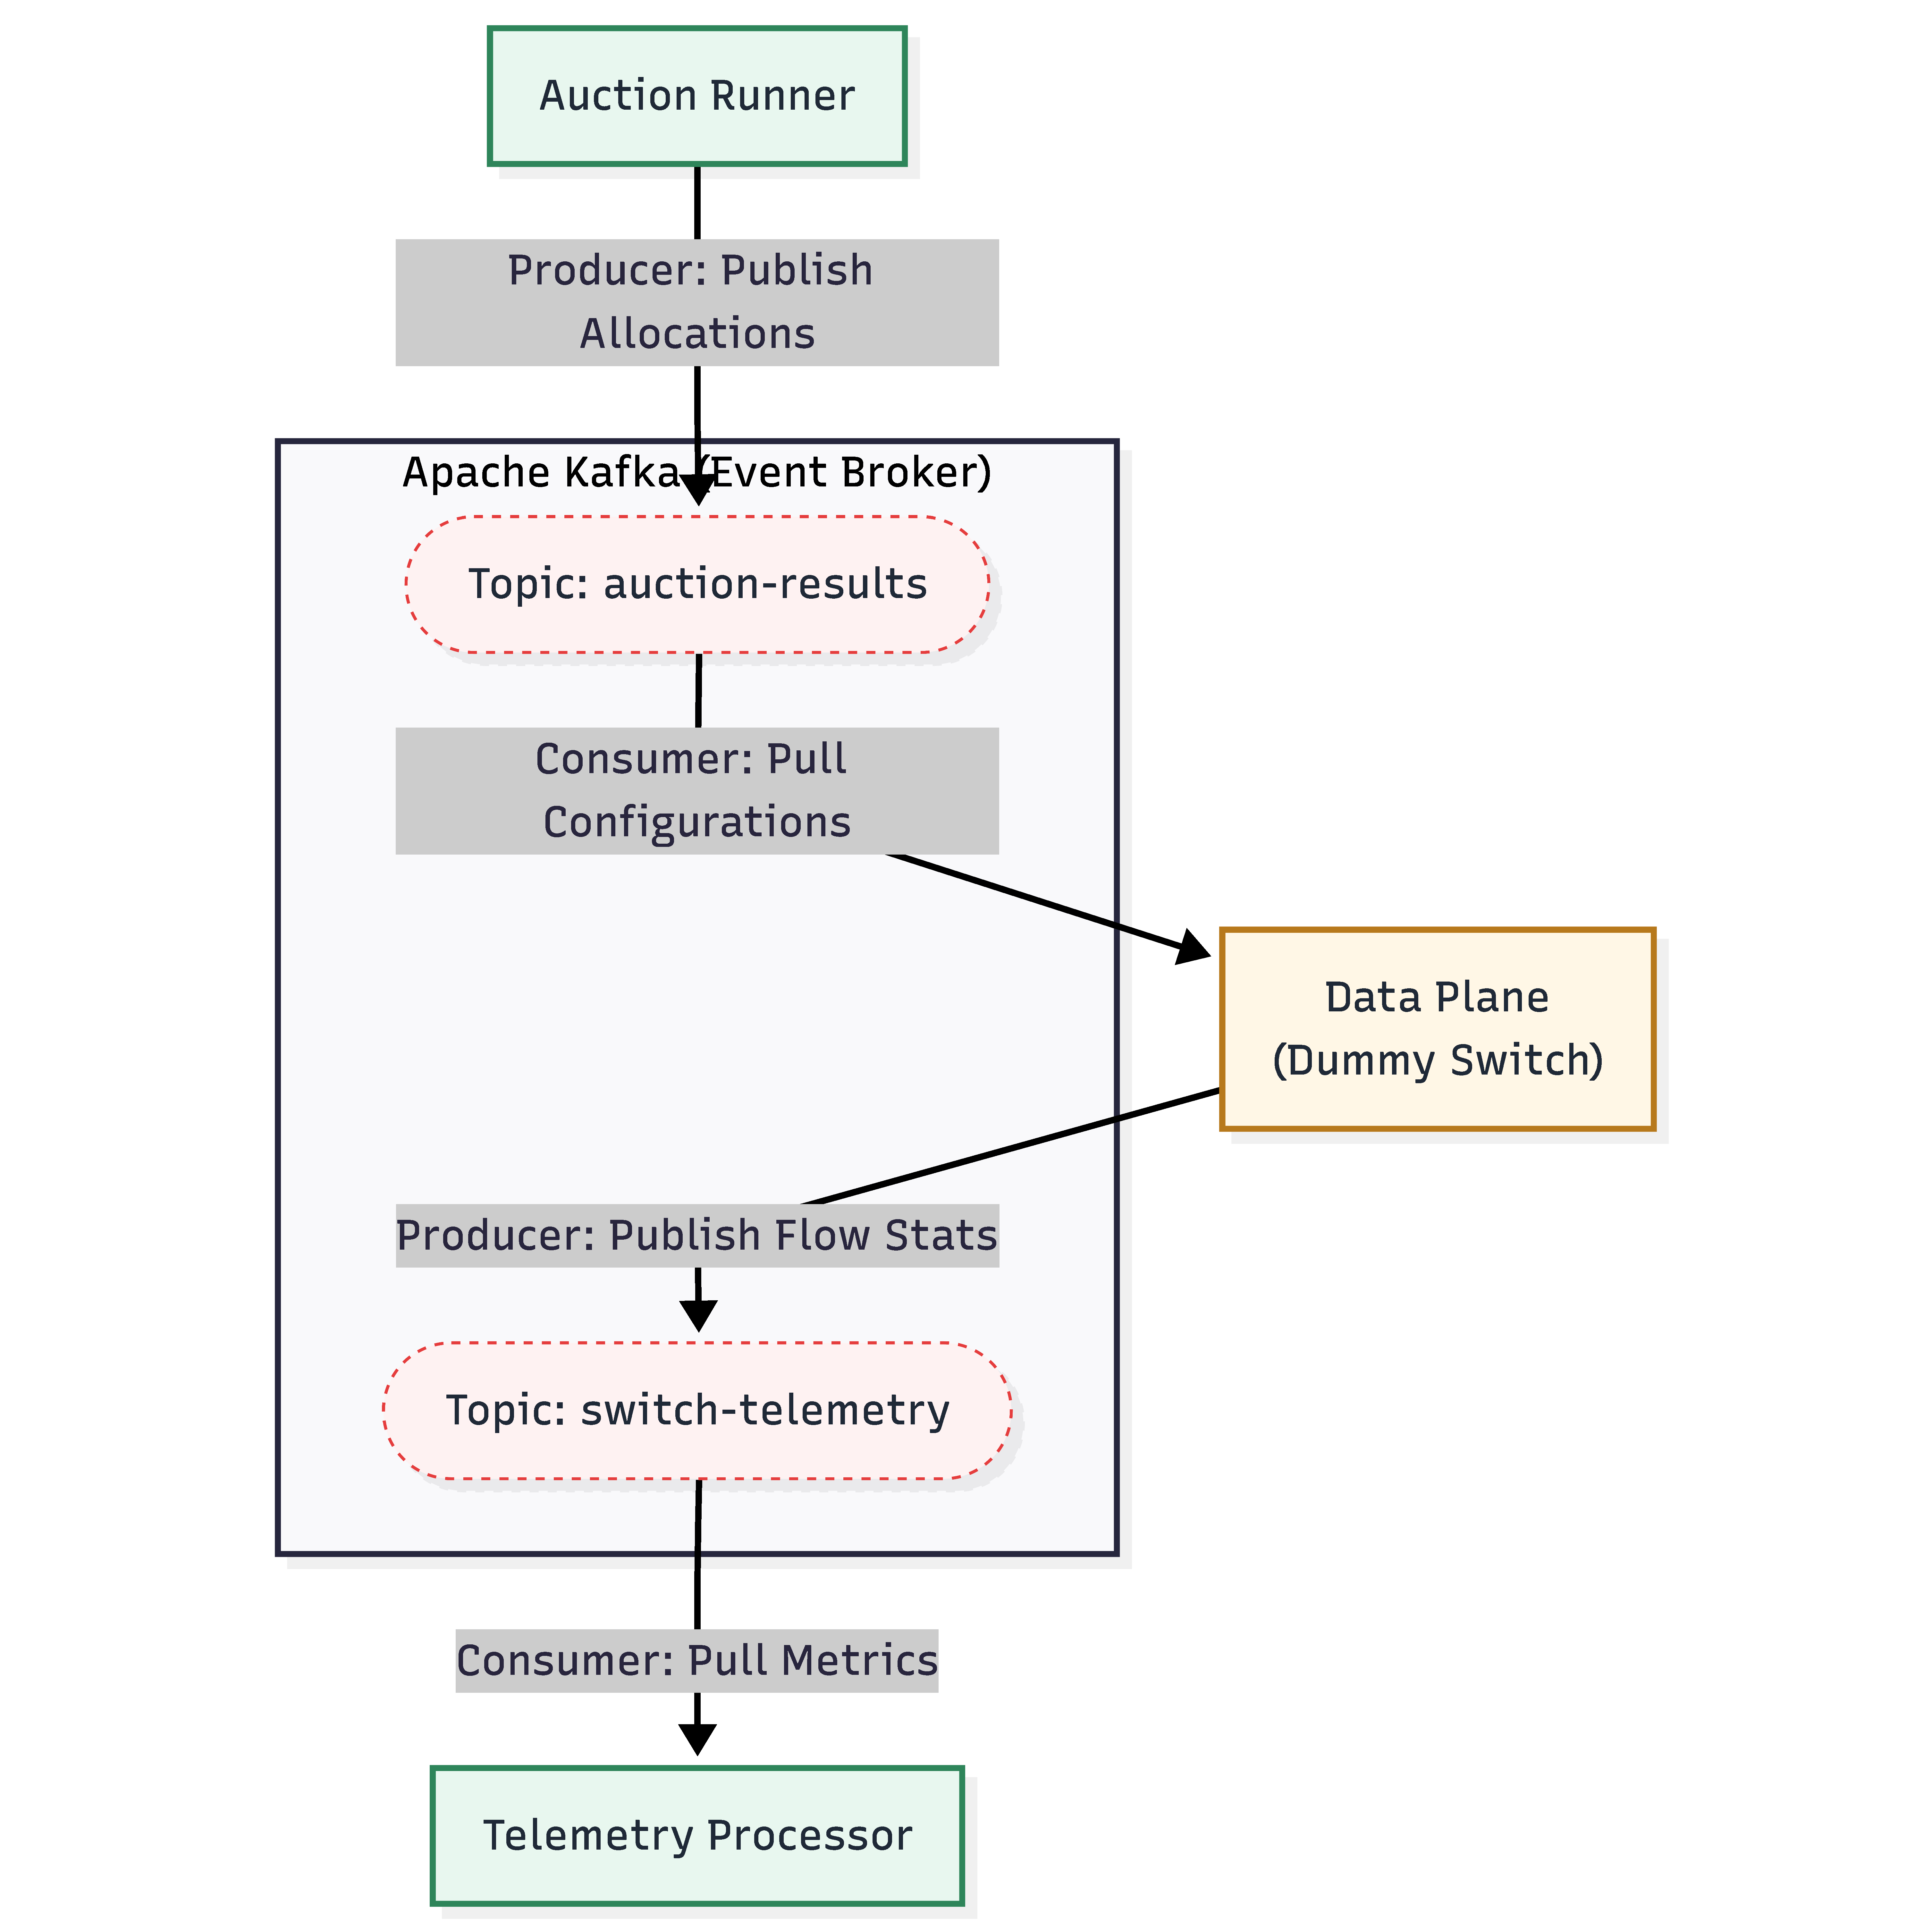
\includegraphics[width=0.85\textwidth]{images/kafka-architecture.pdf}
  \caption{The Publisher/Subscriber decoupling model utilizing Apache Kafka for asynchronous event distribution.}
  \label{fig:kafka_architecture}
\end{figure}

When the Auction Runner completes its clearing algorithm, it publishes final allocations to the \texttt{auction-results} topic. The runner does not wait for the switches to apply these configurations. The data plane agents (represented in testing by the Simulated Switch) act as Consumers, pulling these allocations at their own pace. Conversely, the switches continuously publish high-frequency network metrics to the \texttt{switch-telemetry} topic, which the Telemetry Processor consumes. This publisher/subscriber model isolates failure domains, ensuring that localized data plane degradation does not instantly crash the global control plane.

\section{Control Plane Workflows}

Within this decoupled architecture, the system executes two primary business workflows: the Auction System and the Network Telemetry System. The temporal separation inherent in these workflows is the primary driver for the advanced trace-linking implementation discussed later in this thesis.

\subsection{The Auction System Workflow}
The Auction System handles the ingestion of customer bids and the execution of the economic clearing algorithm. The lifecycle of a bandwidth request is illustrated in Figure~\ref{fig:auction_system}.

\begin{figure}[H]
  \centering
  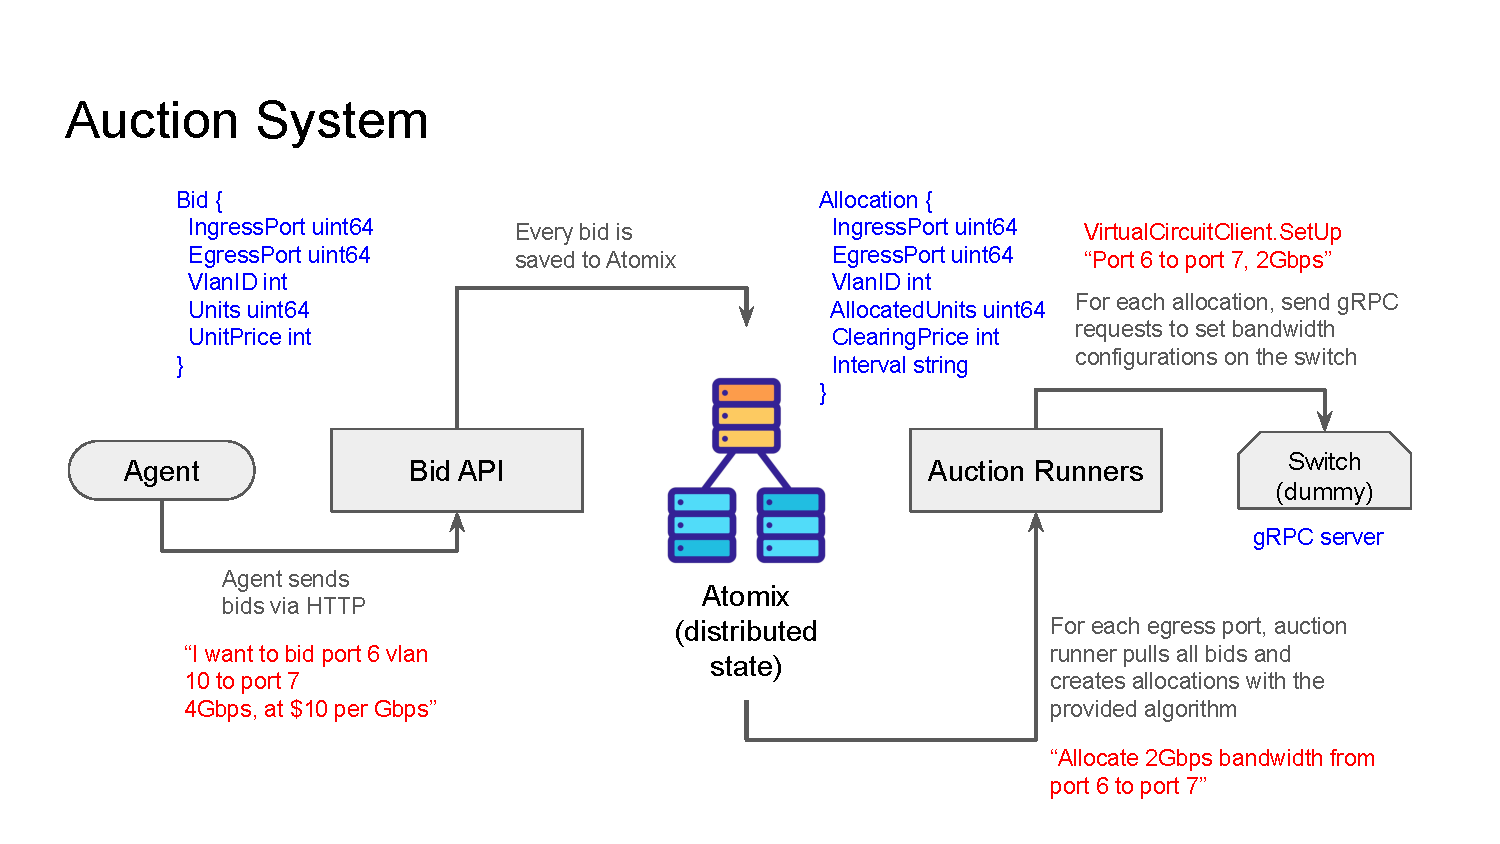
\includegraphics[width=0.95\textwidth]{images/Auction_System.pdf}
  \caption{The Auction System workflow, detailing the path from bid submission to data plane allocation.}
  \label{fig:auction_system}
\end{figure}

Customer agents interface with the API Gateway via HTTP REST endpoints \cite{babalGrpcMicroservicesGo}. A customer submits a \texttt{Bid} payload explicitly defining their \texttt{IngressPort}, \texttt{EgressPort}, \texttt{VlanID}, requested \texttt{Units} (in Kbps), and their maximum \texttt{UnitPrice}. 

Upon receiving a valid request, the API Gateway immediately writes this bid into Atomix. At the scheduled interval, the Auction Runner pulls all accumulated bids for an egress port, executes the uniform-price allocation algorithm, and generates an \texttt{Allocation} record. This record is published to Kafka, where the dummy switch consumes it and simulates data plane enforcement via gRPC (\texttt{VirtualCircuitClient.SetUp}).

\subsection{The Network Telemetry Workflow}
To facilitate a dynamic and competitive marketplace, customer agents must be able to base their bids on real-time network conditions. The Network Telemetry System processes data-plane flow statistics for this purpose, as shown in Figure~\ref{fig:telemetry_system}.

\begin{figure}[H]
  \centering
  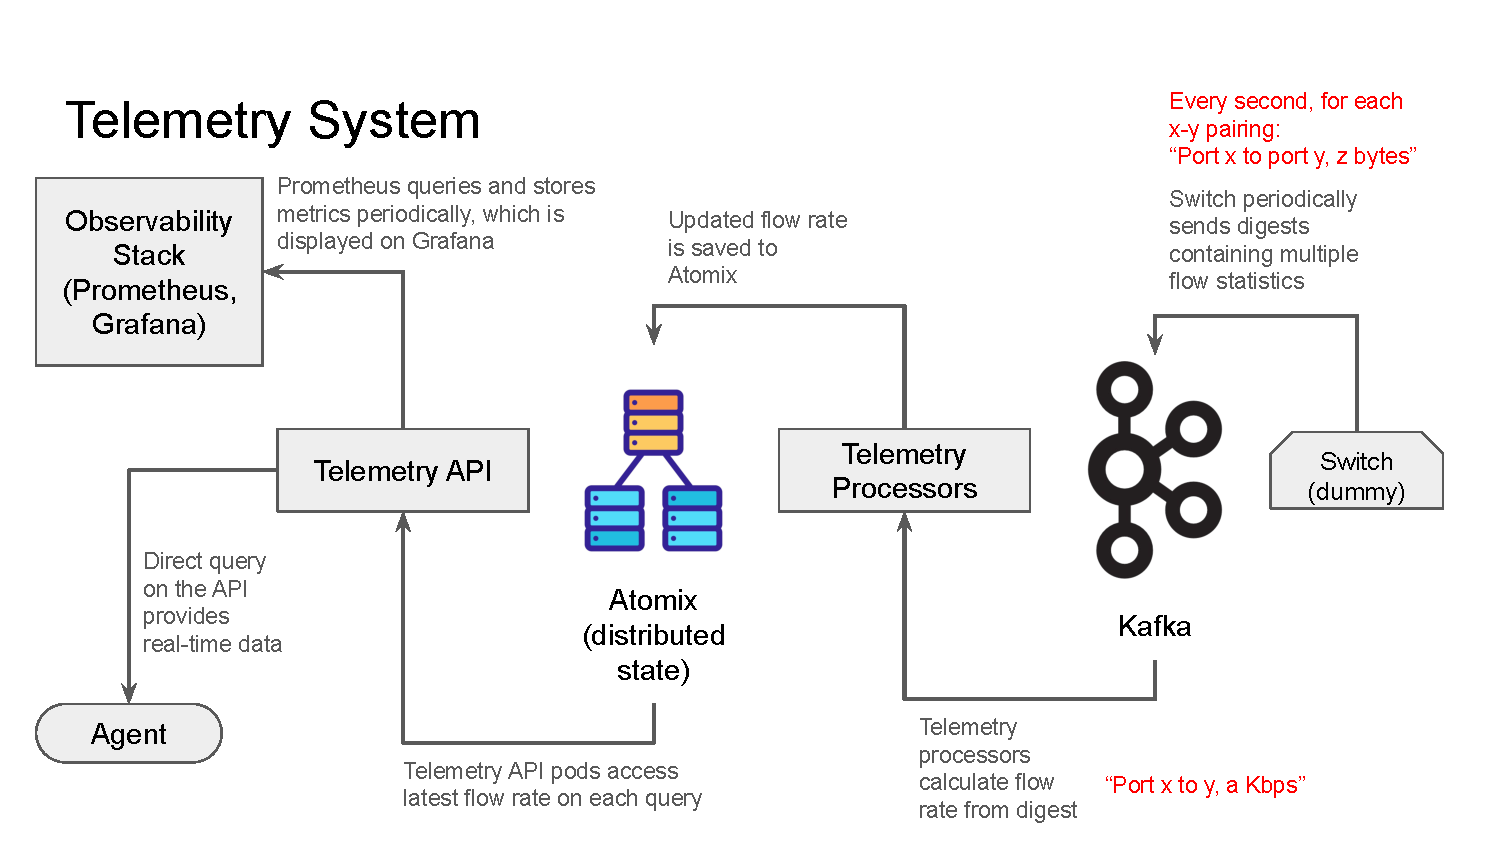
\includegraphics[width=0.95\textwidth]{images/Telemetry_System.pdf}
  \caption{The Network Telemetry workflow, illustrating how raw switch statistics are processed and served to bidding agents.}
  \label{fig:telemetry_system}
\end{figure}

Every second, the Simulated Switch emits a payload containing absolute transfer counts and publishes it to the \texttt{switch-telemetry} topic. The Telemetry Processor microservices continuously consume these counts, perform windowed calculations to convert them into standardized flow rates (Kbps), and update the corresponding network state records within Atomix. When a Customer Agent prepares to bid, it executes an HTTP GET query against the API Gateway's Telemetry API to retrieve this real-time snapshot of network congestion.

\section{Summary}

This chapter presented the complete system architecture and data workflows for the SDN global control plane. The microservice design utilizes Atomix for consistent state management and Kafka for asynchronous hardware decoupling. The detailed Auction and Telemetry workflows demonstrate exactly how customer intent is transformed into network reality. 

However, because these workflows are temporally decoupled—where a bid is written by one service and read by another service a full minute later—traditional monitoring tools lose track of the request lifecycle. The next chapter explores the specific implementation logic behind these workflows, providing the foundation necessary to understand how the custom observability framework solves this asynchronous tracking problem.